\newif\ifshowsolutions
\showsolutionstrue

% SWITCH IF USING OVERLEAF
%\documentclass{article}
\usepackage{listings}
\usepackage{amsmath}
\usepackage{subfig}
\usepackage{amsthm}
\usepackage{amsmath}
\usepackage{amssymb}
\usepackage{graphicx}
\usepackage{mdwlist}
\usepackage{geometry}
\usepackage{titlesec}
\usepackage{palatino}
\usepackage{mathrsfs}
\usepackage{fancyhdr}
\usepackage{paralist}
\usepackage{todonotes}
\usepackage{tikz}
\usepackage{float} % Place figures where you ACTUALLY want it
\usepackage{comment} % A hack to toggle sections
\usepackage{ifthen}
\usepackage{mdframed}
\usepackage{verbatim}
\usepackage{listings}
\usepackage{bbm}
\usepackage{upquote} % Prevents backticks replacing single-quotes in verbatim
\usepackage[strings]{underscore}
\usepackage[colorlinks=true]{hyperref}
\usetikzlibrary{positioning,shapes,backgrounds}

\geometry{margin=1in}
\geometry{headheight=2in}
\geometry{top=2in}

\setlength{\marginparwidth}{2.15cm}
\setlength{\parindent}{0em}
\setlength{\parskip}{0.6\baselineskip}

\rhead{}
\lhead{}

% Spacing settings.
\titlespacing\section{0pt}{12pt plus 2pt minus 2pt}{0pt plus 2pt minus 2pt}
\titlespacing\subsection{0pt}{12pt plus 4pt minus 2pt}{0pt plus 2pt minus 2pt}
\titlespacing\subsubsection{0pt}{12pt plus 4pt minus 2pt}{0pt plus 2pt minus 2pt}
\renewcommand{\baselinestretch}{1.15}

% Shortcuts for commonly used operators.
\newcommand{\E}{\mathbb{E}}
\newcommand{\Var}{\operatorname{Var}}
\newcommand{\Cov}{\operatorname{Cov}}
\newcommand{\Bias}{\operatorname{Bias}}
\DeclareMathOperator{\argmin}{arg\,min}
\DeclareMathOperator{\argmax}{arg\,max}

% Do not number subsections and below.
\setcounter{secnumdepth}{1}

% Custom format subsection.
\titleformat*{\subsection}{\large\bfseries}

% Set up the problem environment.
\newcounter{problem}[section]
\newenvironment{problem}[1][]
  {\begingroup
    \setlength{\parskip}{0em}
    \refstepcounter{problem}\par\addvspace{1em}\textbf{Problem~\Alph{problem}\!
    \ifthenelse{\equal{#1}{}}{}{ [#1 points]}:}
  \endgroup}

% Set up the subproblem environment.
\newcounter{subproblem}[problem]
\newenvironment{subproblem}[1][]
  {\begingroup
    \setlength{\parskip}{0em}
    \refstepcounter{subproblem}\par\medskip\textbf{\roman{subproblem}.\!
    \ifthenelse{\equal{#1}{}}{}{ [#1 points]:}}
  \endgroup}

% Set up the teachers and materials commands.
\newcommand\teachers[1]
  {\begingroup
    \setlength{\parskip}{0em}
    \vspace{0.3em} \textit{\hspace*{2em} TAs responsible: #1} \par
  \endgroup}
\newcommand\materials[1]
  {\begingroup
    \setlength{\parskip}{0em}
    \textit{\hspace*{2em} Relevant materials: #1} \par \vspace{1em}
  \endgroup}

% Set up the hint environment.
\newenvironment{hint}[1][]
  {\begin{em}\textbf{Hint: }}
  {\end{em}}


% Set up the solution environment.
\ifshowsolutions
  \newenvironment{solution}[1][]
    {\par\medskip \begin{mdframed}\textbf{Solution~\Alph{problem}#1:} \begin{em}}
    {\end{em}\medskip\end{mdframed}\medskip}
  \newenvironment{subsolution}[1][]
    {\par\medskip \begin{mdframed}\textbf{Solution~\Alph{problem}#1.\roman{subproblem}:} \begin{em}}
    {\end{em}\medskip\end{mdframed}\medskip}
\else
  \excludecomment{solution}
  \excludecomment{subsolution}
\fi

\documentclass{article}
\usepackage{listings}
\usepackage{amsmath}
\usepackage{subfig}
\usepackage{amsthm}
\usepackage{amsmath}
\usepackage{amssymb}
\usepackage{graphicx}
\usepackage{mdwlist}
\usepackage{geometry}
\usepackage{titlesec}
\usepackage{palatino}
\usepackage{mathrsfs}
\usepackage{fancyhdr}
\usepackage{paralist}
\usepackage{todonotes}
\usepackage{tikz}
\usepackage{float} % Place figures where you ACTUALLY want it
\usepackage{comment} % A hack to toggle sections
\usepackage{ifthen}
\usepackage{mdframed}
\usepackage{verbatim}
\usepackage{listings}
\usepackage{bbm}
\usepackage{upquote} % Prevents backticks replacing single-quotes in verbatim
\usepackage[strings]{underscore}
\usepackage[colorlinks=true]{hyperref}
\usetikzlibrary{positioning,shapes,backgrounds}

\geometry{margin=1in}
\geometry{headheight=2in}
\geometry{top=2in}

\setlength{\marginparwidth}{2.15cm}
\setlength{\parindent}{0em}
\setlength{\parskip}{0.6\baselineskip}

\rhead{}
\lhead{}

% Spacing settings.
\titlespacing\section{0pt}{12pt plus 2pt minus 2pt}{0pt plus 2pt minus 2pt}
\titlespacing\subsection{0pt}{12pt plus 4pt minus 2pt}{0pt plus 2pt minus 2pt}
\titlespacing\subsubsection{0pt}{12pt plus 4pt minus 2pt}{0pt plus 2pt minus 2pt}
\renewcommand{\baselinestretch}{1.15}

% Shortcuts for commonly used operators.
\newcommand{\E}{\mathbb{E}}
\newcommand{\Var}{\operatorname{Var}}
\newcommand{\Cov}{\operatorname{Cov}}
\newcommand{\Bias}{\operatorname{Bias}}
\DeclareMathOperator{\argmin}{arg\,min}
\DeclareMathOperator{\argmax}{arg\,max}

% Do not number subsections and below.
\setcounter{secnumdepth}{1}

% Custom format subsection.
\titleformat*{\subsection}{\large\bfseries}

% Set up the problem environment.
\newcounter{problem}[section]
\newenvironment{problem}[1][]
  {\begingroup
    \setlength{\parskip}{0em}
    \refstepcounter{problem}\par\addvspace{1em}\textbf{Problem~\Alph{problem}\!
    \ifthenelse{\equal{#1}{}}{}{ [#1 points]}:}
  \endgroup}

% Set up the subproblem environment.
\newcounter{subproblem}[problem]
\newenvironment{subproblem}[1][]
  {\begingroup
    \setlength{\parskip}{0em}
    \refstepcounter{subproblem}\par\medskip\textbf{\roman{subproblem}.\!
    \ifthenelse{\equal{#1}{}}{}{ [#1 points]:}}
  \endgroup}

% Set up the teachers and materials commands.
\newcommand\teachers[1]
  {\begingroup
    \setlength{\parskip}{0em}
    \vspace{0.3em} \textit{\hspace*{2em} TAs responsible: #1} \par
  \endgroup}
\newcommand\materials[1]
  {\begingroup
    \setlength{\parskip}{0em}
    \textit{\hspace*{2em} Relevant materials: #1} \par \vspace{1em}
  \endgroup}

% Set up the hint environment.
\newenvironment{hint}[1][]
  {\begin{em}\textbf{Hint: }}
  {\end{em}}


% Set up the solution environment.
\ifshowsolutions
  \newenvironment{solution}[1][]
    {\par\medskip \begin{mdframed}\textbf{Solution~\Alph{problem}#1:} \begin{em}}
    {\end{em}\medskip\end{mdframed}\medskip}
  \newenvironment{subsolution}[1][]
    {\par\medskip \begin{mdframed}\textbf{Solution~\Alph{problem}#1.\roman{subproblem}:} \begin{em}}
    {\end{em}\medskip\end{mdframed}\medskip}
\else
  \excludecomment{solution}
  \excludecomment{subsolution}
\fi




%%%%%%%%%%%%%%%%%%%%%%%%%%%%%%
% HEADER
%%%%%%%%%%%%%%%%%%%%%%%%%%%%%%

\chead{
  {\vbox{
      \vspace{2mm}
      \large
      Machine Learning \& Data Mining \hfill
      Caltech CS/CNS/EE 155 \hfill \\[1pt]
      Set 3\hfill
      February $2^\text{nd}$, 2023 \\
      Got a 2 Day Extension from Professor Lee \hfill
      Manuel Rodriguez \\
    }
  }
}

\begin{document}
\pagestyle{fancy}



%%%%%%%%%%%%%%%%%%%%%%%%%%%%%%
% POLICIES
%%%%%%%%%%%%%%%%%%%%%%%%%%%%%%

\section*{Policies}
\begin{itemize}
	\item Due 9 PM PST, January $31^\text{th}$ on Gradescope. 
	\item You are free to collaborate on all of the problems, subject to the collaboration policy stated in the syllabus.
	\item In this course, we will be using Google Colab for code submissions. You will need a Google account.
\end{itemize}

\section*{Submission Instructions}
\begin{itemize}
	\item Submit your report as a single .pdf file to Gradescope, under "Set 3 Report". 
	\item In the report, \textbf{include any images generated by your code} along with your answers to the questions.
	\item Submit your code by \textbf{sharing a link in your report} to your Google Colab notebook for each problem (see naming instructions below). Make sure to set sharing permissions to at least "Anyone with the link can view". \textbf{Links that can not be run by TAs will not be counted as turned in.} Check your links in an incognito window before submitting to be sure. 
	\item For instructions specifically pertaining to the Gradescope submission process, see \url{https://www.gradescope.com/get_started#student-submission}.
\end{itemize}

\section*{Google Colab Instructions}
For each notebook, you need to save a copy to your drive.
\begin{enumerate}
	\item Open the github preview of the notebook, and click the icon to open the colab preview.
	\item On the colab preview, go to File $\rightarrow$ Save a copy in Drive.
	\item Edit your file name to “lastname_firstname_set_problem”, e.g.”yue_yisong_set3_prob2.ipynb”
\end{enumerate}

%%%%%%%%%%%%%%%%%%%%%%%%%%%%%%
% PROBLEM 1
%%%%%%%%%%%%%%%%%%%%%%%%%%%%%%

\newpage
\section{Decision Trees [30 Points]}
\materials{Lecture 5}

\problem[7]
Consider the following data, where given information about some food you must predict whether it is healthy:

\begin{table}[ht]
\centering
\begin{tabular}{c | c c c | c}
\hline
No. & Package Type & Unit Price $>$ \$5 & Contains $>$ 5 grams of fat & Healthy? \\ [0.5ex]
\hline
1 & Canned & Yes & Yes & No  \\
2 & Bagged & Yes & No  & Yes \\
3 & Bagged & No  & Yes & Yes \\
4 & Canned & No  & No  & Yes \\ [1ex]
\hline
\end{tabular}
\end{table}

Train a decision tree by hand using top-down greedy induction. Use \emph{entropy} (with natural log) as the impurity measure.  Since the data can be classified
without error, the stopping criterion will be no impurity in the leaves.

Submit a drawing of your tree showing the impurity reduction yielded by each split (including root) in your decision tree.

\begin{solution}
    \\
    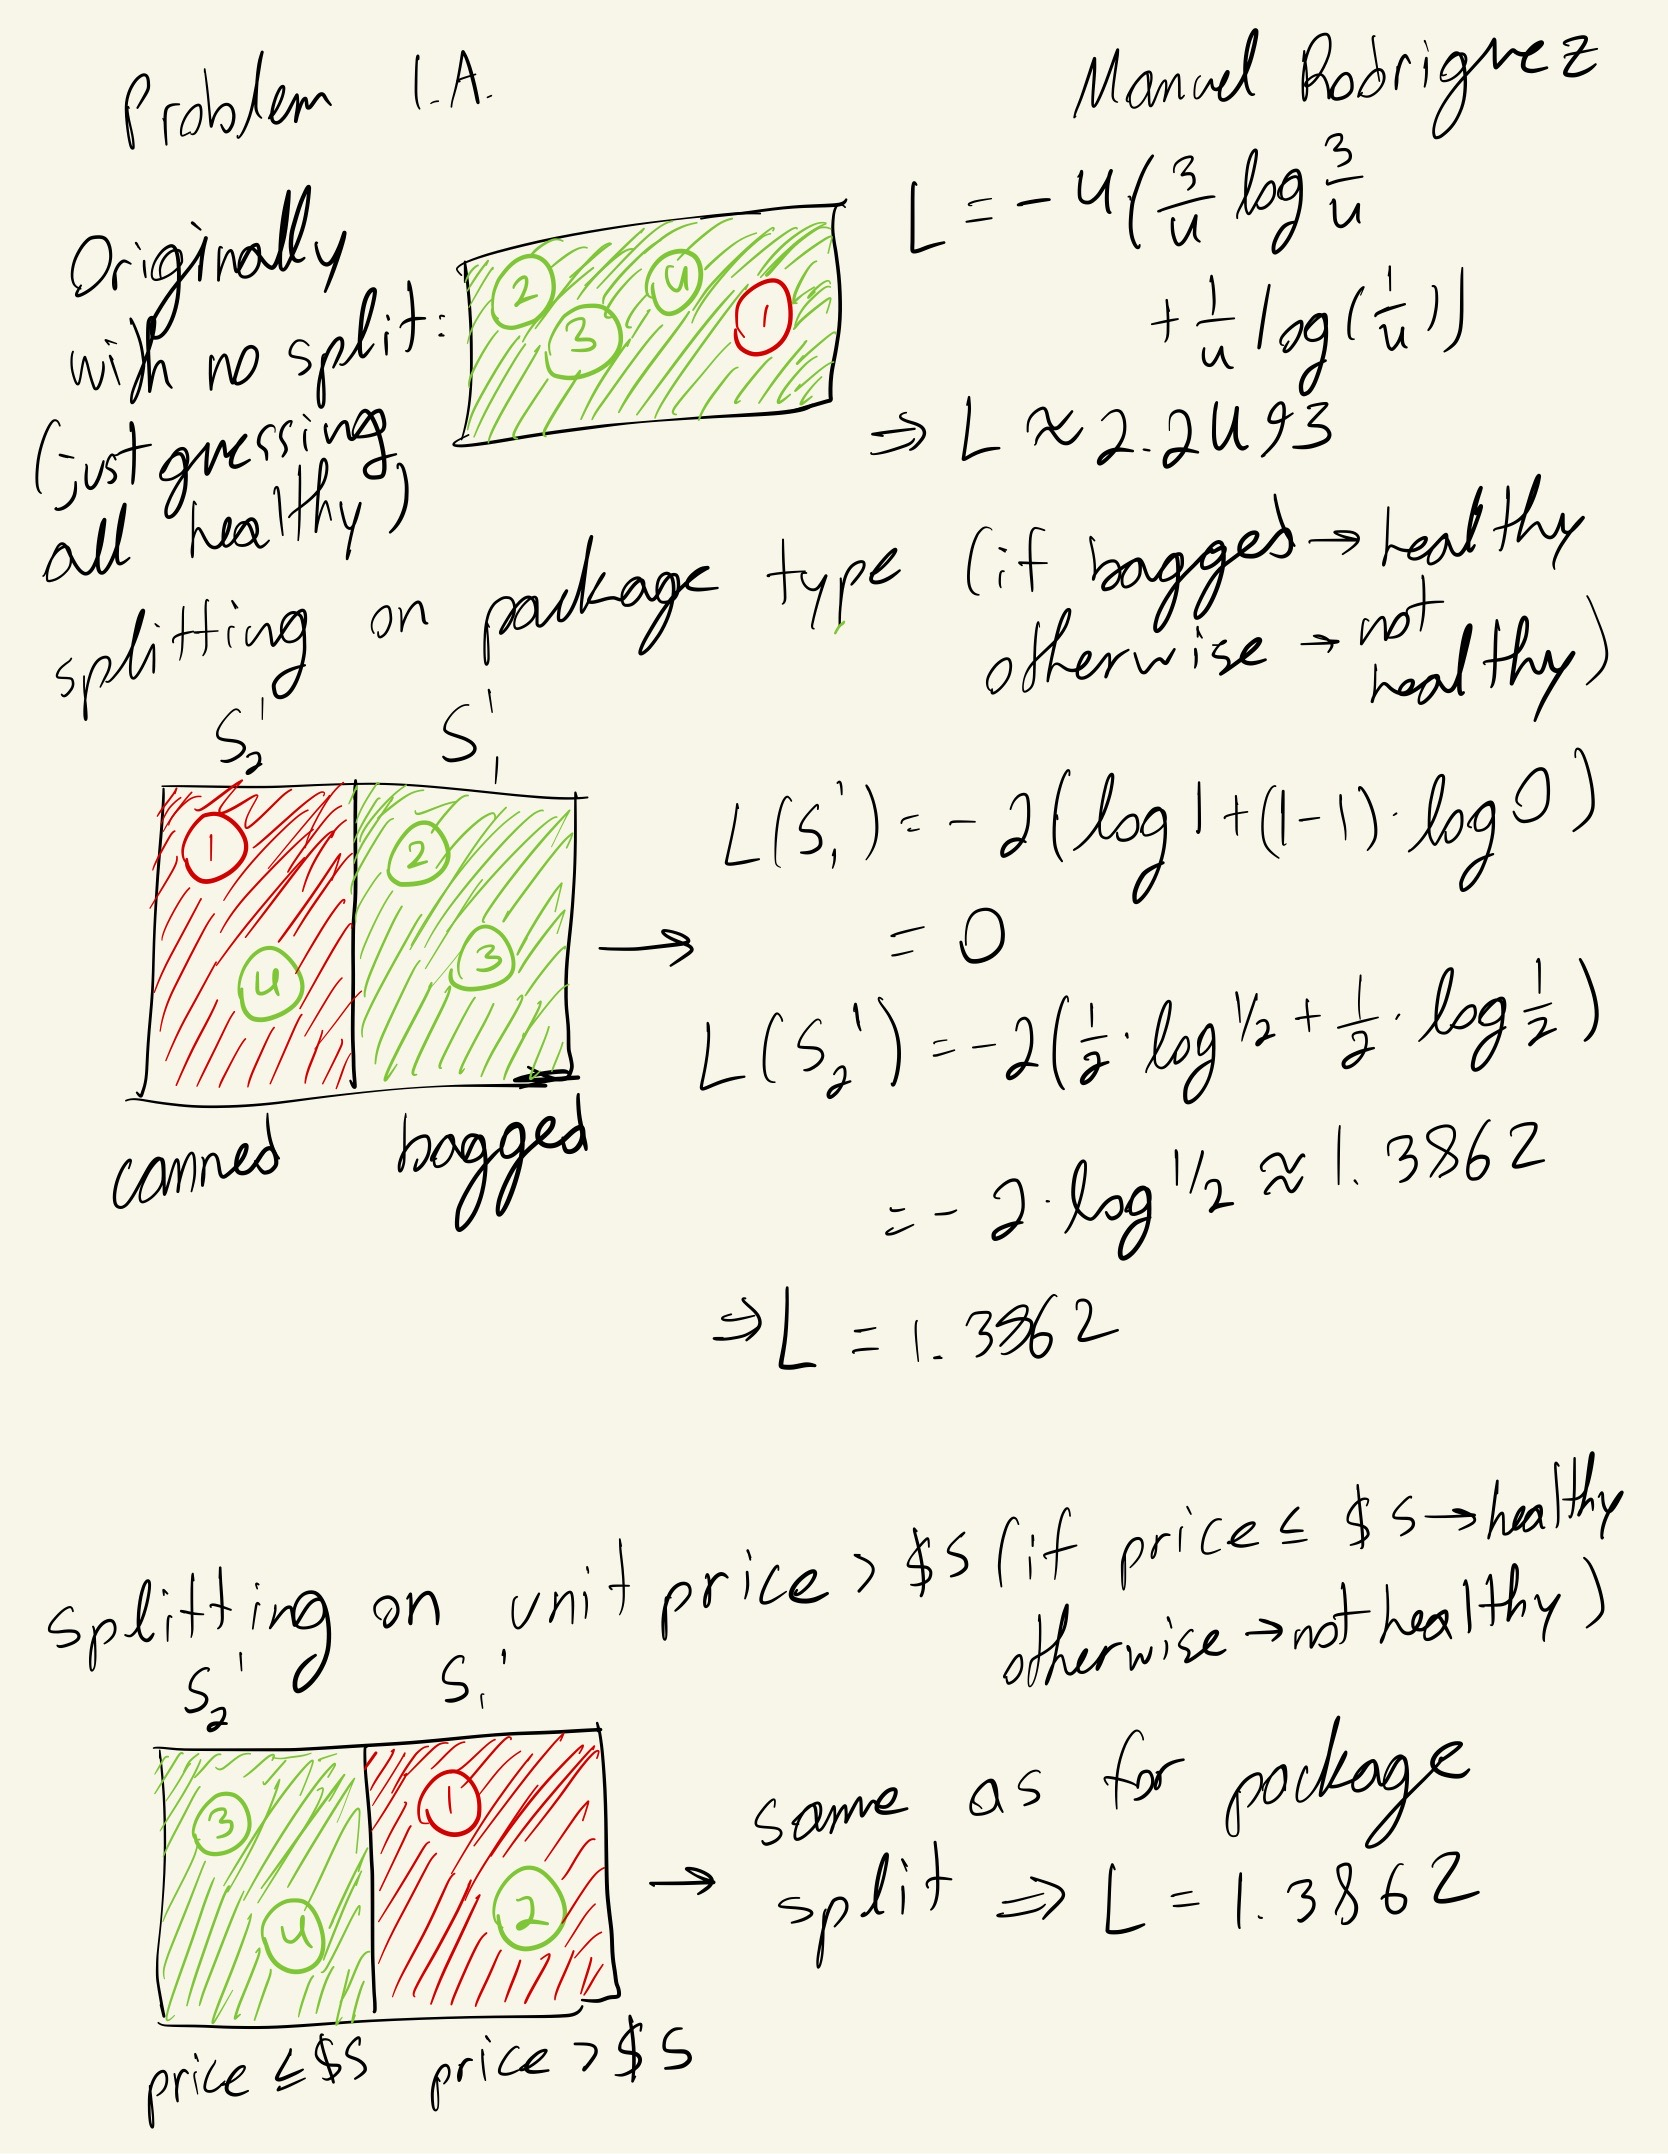
\includegraphics[width=12cm]{images/P1_A_1.JPG} \\
    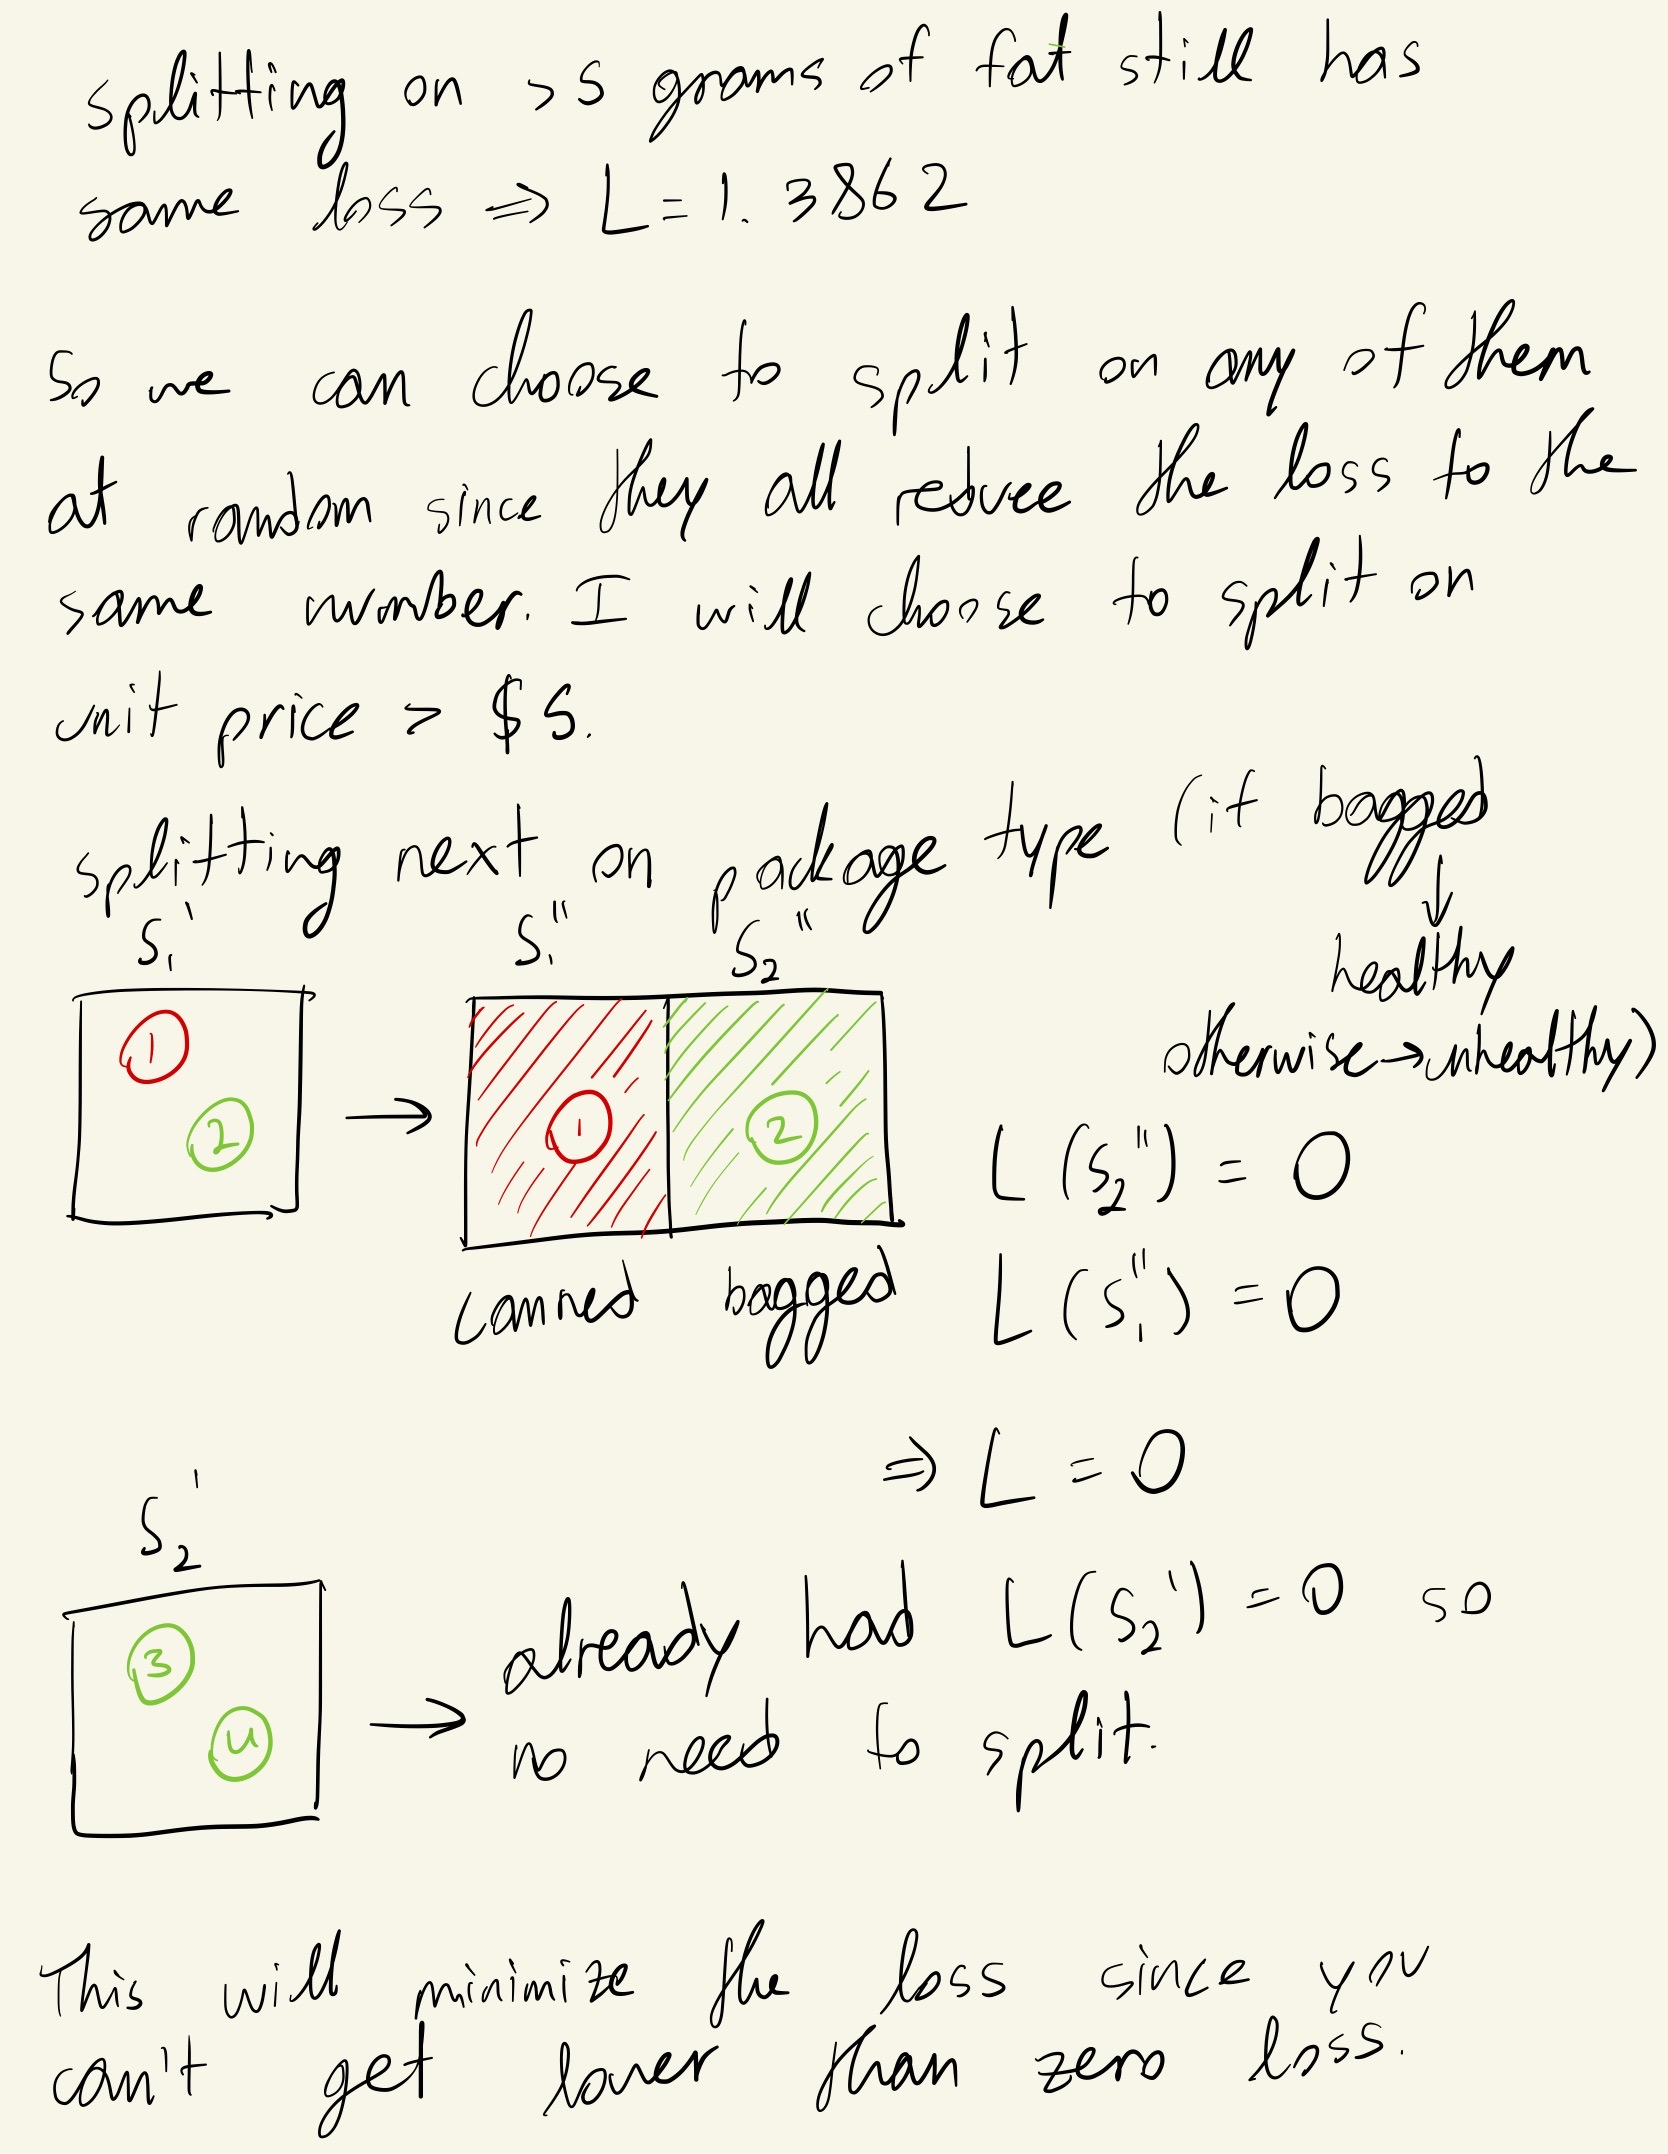
\includegraphics[width=12cm]{images/P1_A_2.JPG} \\
    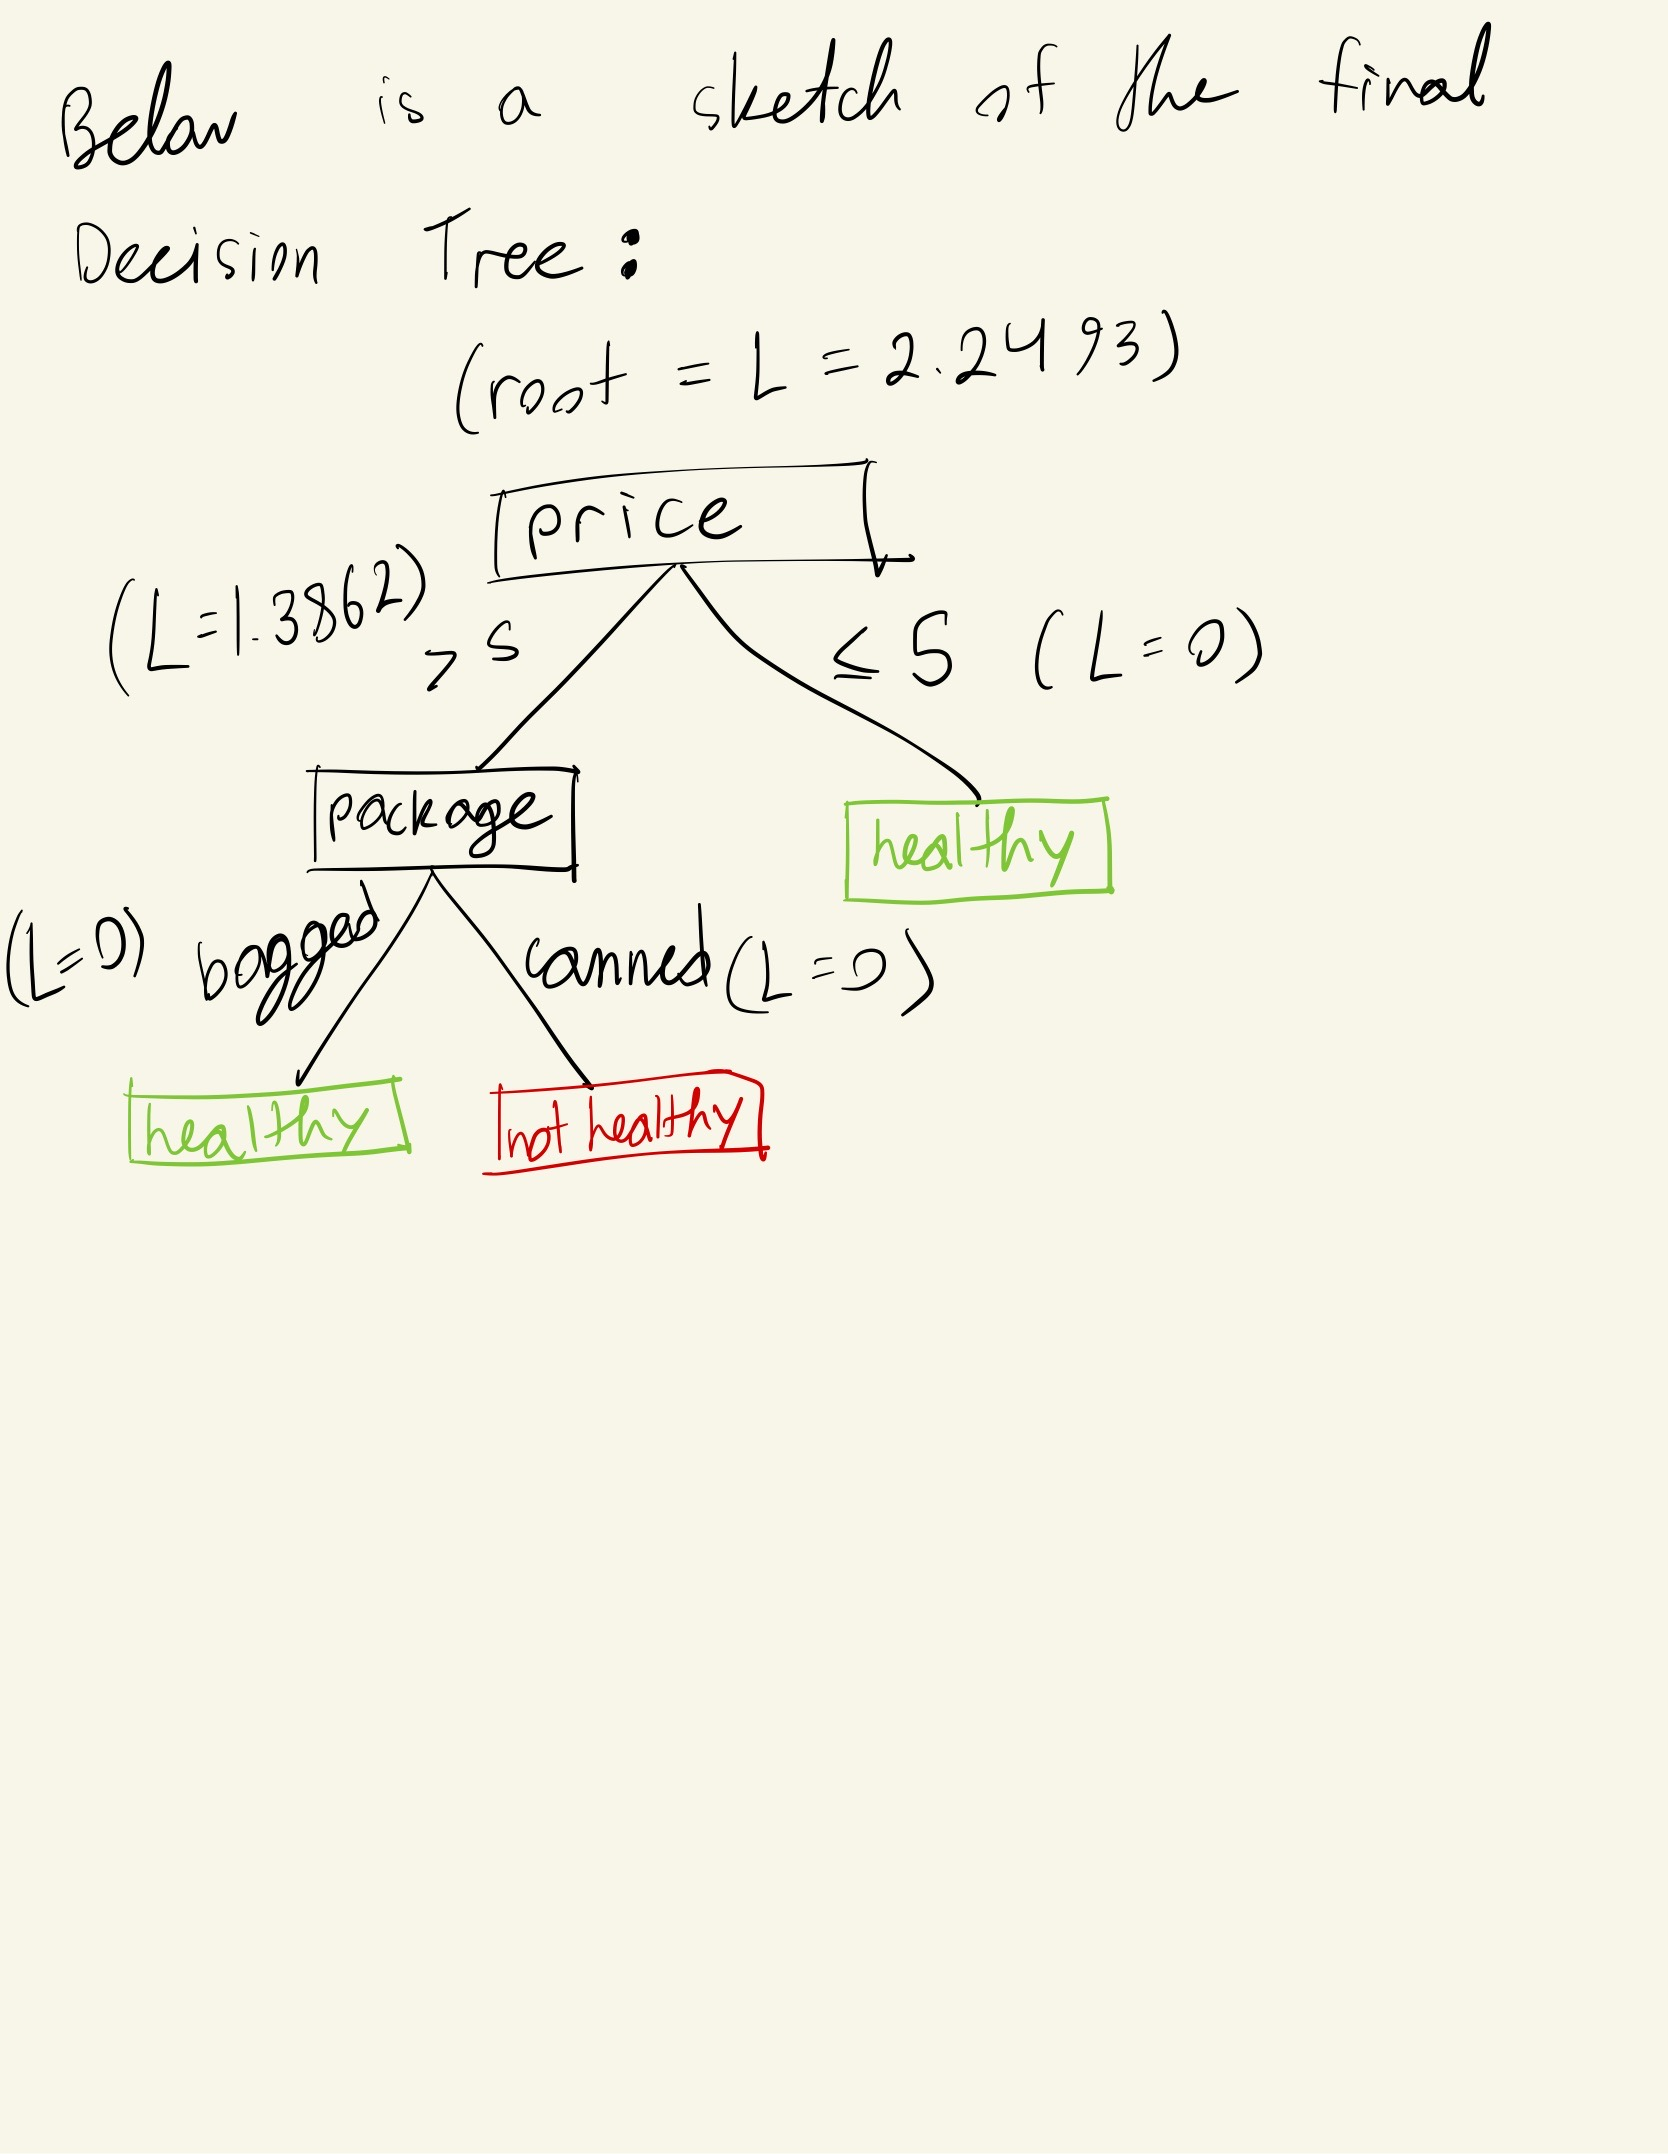
\includegraphics[width=12cm]{images/P1_A_3.JPG} \\
\end{solution}

\problem[4]
Compared to a linear classifier, is a decision tree always preferred for classification problems? Briefly explain why or why not. If not, draw a simple 2-D dataset that can be perfectly classified by a simple linear classifier but which requires an overly complex decision tree to perfectly classify.

\begin{solution}
  A linear classifier is can be preferred to a decision tree when the data being observed is linearly separable or linearly separable plus some noise (fixed with regularization). A decision tree would need to be overly complex to account for diagonal separation in terms of the axes whereas a simple linear model could readily separate the data. Because this decision tree would be overly complex and decision trees in general are prone to overfitting, this decision tree would likely perform poorly on the out of sample data. Below is an example of a dataset (taken from the class lecture slides) that is simple to model using linear models but complex with decision trees: \\
  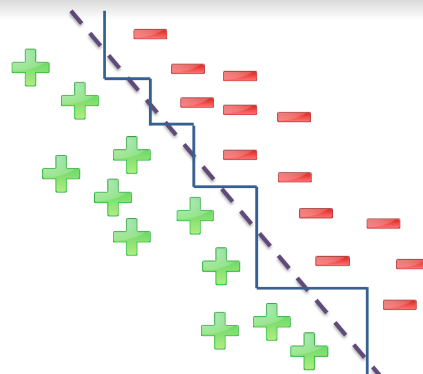
\includegraphics{images/P1_b.png} \\
\end{solution}

\problem[15]
Consider the following 2D data set:
\begin{figure}[H]
    \begin{center}
    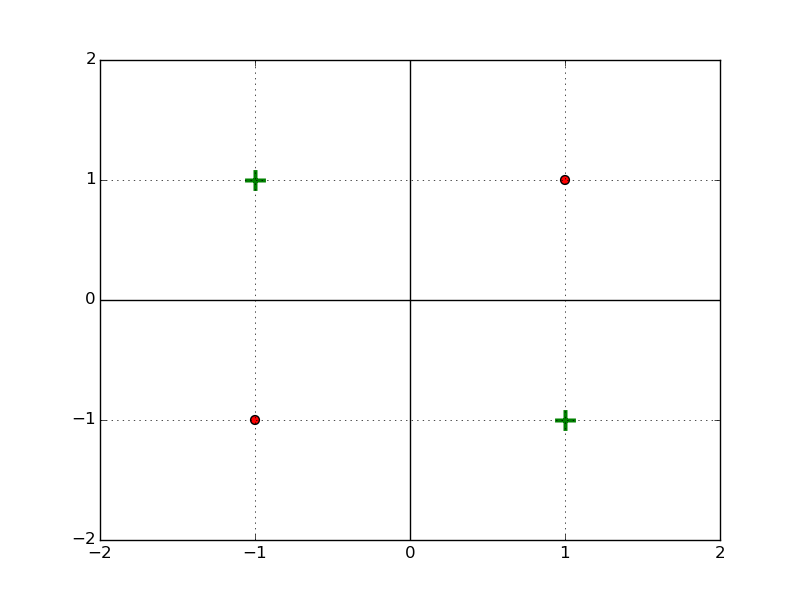
\includegraphics[width=3.3in]{plots/3C.png}
    \end{center}
    \end{figure}

\subproblem[5] Suppose we train a decision tree on this dataset using top-down greedy induction, with the Gini index as
the impurity measure. We define our stopping condition to be if no split of a node
results in any reduction in impurity. Submit a drawing of the resulting tree.  What is its classification error ((number of misclassified points) / (number of total points))?

\subproblem[5] Submit a drawing of a two-level decision tree that classifies the above dataset with zero classification error.  (You don't need to use any particular training algorithm to produce the tree.)

Is there any impurity measure (i.e. any function that maps the data points under a particular node in a tree to a real number) that would have led top-down greedy induction with the same stopping condition to produce the tree you drew?  If so, give an example of one, and briefly describe its pros and cons as an impurity measure for training decision trees in general (on arbitrary datasets). 

\subproblem[5] Suppose there are 100 data points in some 2-D dataset. What is the largest number of unique thresholds (i.e., internal nodes) you might need in order to achieve zero classification training error (on the training set)? Please
justify your answer.

\begin{solution}
    \\
    ii. \\
    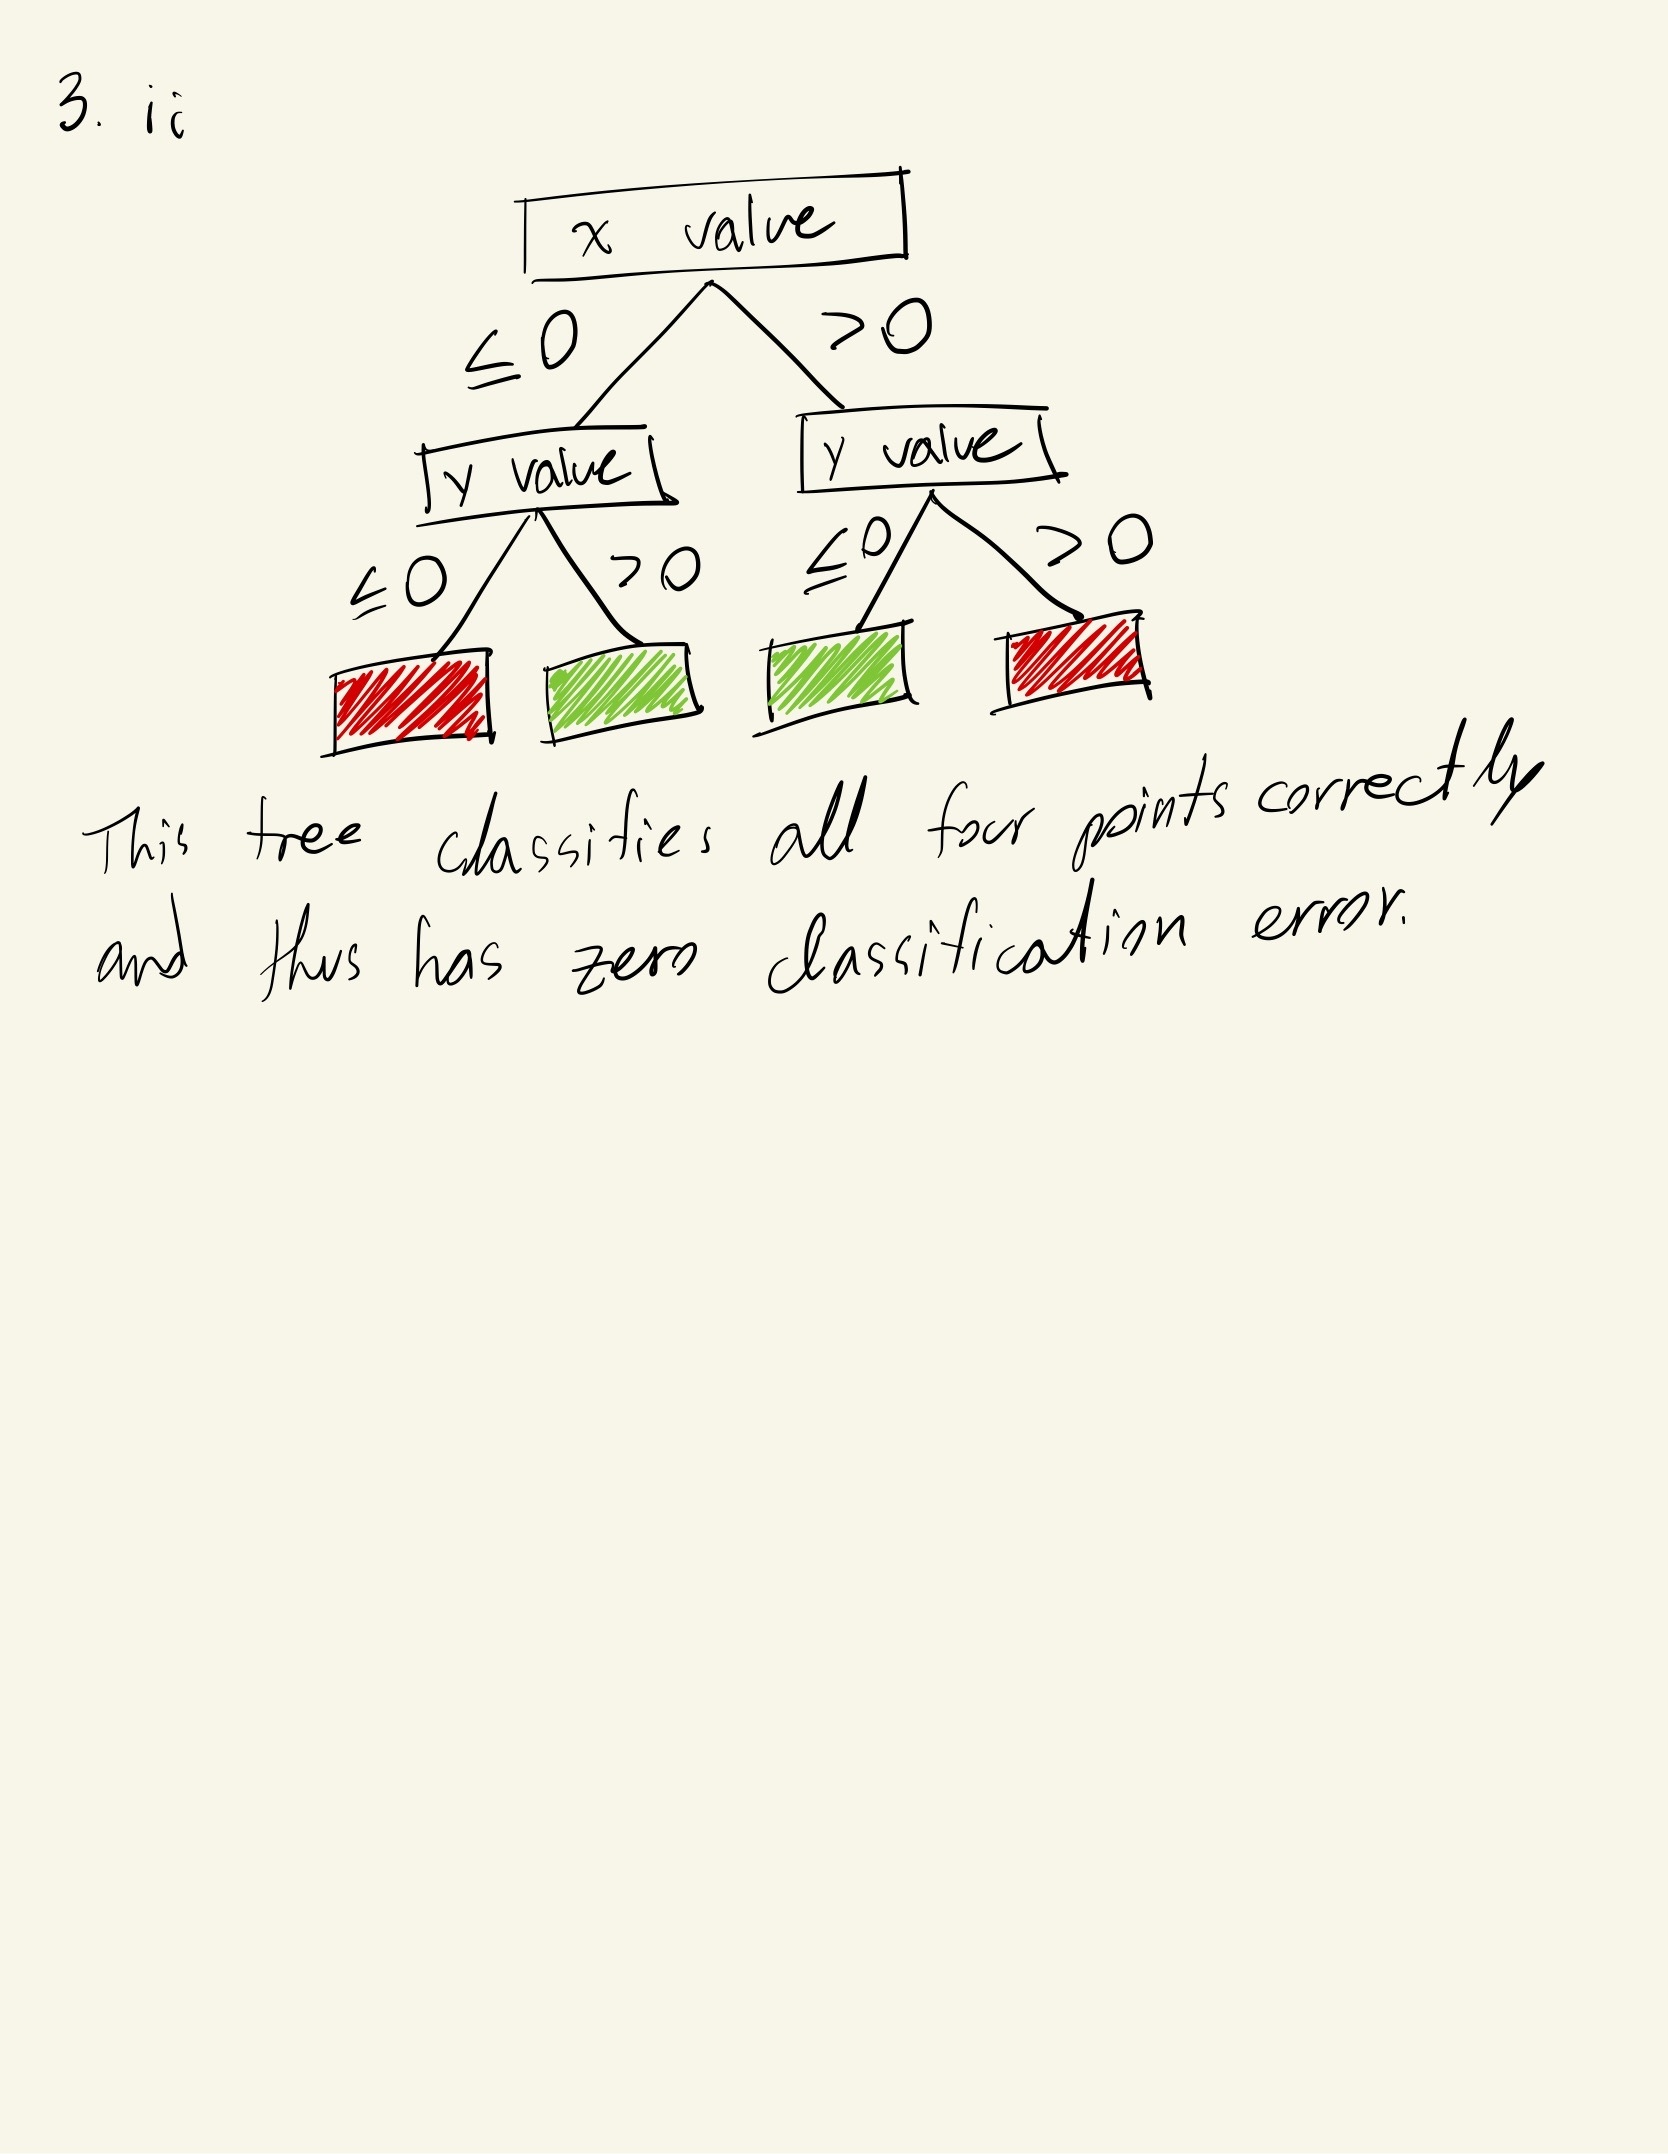
\includegraphics[width=9.5cm]{images/P1_C_ii.JPG} \\
    iii. If there are 100 data points, the worst case scenario is that all the points are in a line along some axis and they are of alternating classification. For this, we would need 99 decision tree thresholds (one between each pair of consecutive points) to distinguish between them all.
\end{solution}

\problem[4] Suppose in top-down greedy induction we want to split a leaf node that contains N data points composed of
D continuous features. What is the worst-case
complexity (big-O in terms of N and D) of the number of possible splits we must consider in order to find the one that most reduces impurity? Please justify your answer.

Note: Recall that at each node-splitting step in training a DT, you must consider all possible splits that you can make. While there are an infinite number of possible decision boundaries since we are using continuous features, there are not an infinite number of boundaries that result in unique child sets (which is what we mean by ``split'').

\begin{solution}
   In the worst case, the maximum number of splits (as mentioned in lecture) is equal to: \\
   $(\text{\# data points}) \times (\text{\# features per data point}) = N \cdot D$ \\
   This makes sense because for each data point, there are $D$ possible features that could be used for splitting and the number of data points determines how much each of these features can separate the data (since many feature splits can result in the same child sets and thus are equivalent when determining training error).
\end{solution}

%%%%%%%%%%%%%%%%%%%%%%%%%%%%%%
% PROBLEM 2
%%%%%%%%%%%%%%%%%%%%%%%%%%%%%%

\newpage

\section{Overfitting Decision Trees [30 Points, EC 7 Points]}
\materials{Lecture 5}

In this problem, you will use the Diabetic Retinopathy Debrecen Data Set, which contains features extracted from images to determine whether or not the images contain signs of diabetic retinopathy. Additional information about this dataset can be found at the link below:

\url{https://archive.ics.uci.edu/ml/datasets/Diabetic+Retinopathy+Debrecen+Data+Set}

In the following question, your goal is to predict the diagnosis of diabetic retinopathy, which is the final column in the data matrix.  Use the first 900 rows as training data, and the last
251 rows as validation data. Please feel free to use additional packages such as Scikit-Learn. Include your code in your submission.


\indent\problem[10] \smallskip 
Choose one of the following from i or ii: 

\noindent i. Train a decision tree classifier using Gini as the impurity measure and minimal leaf node size as early stopping criterion. Try different minimal leaf node sizes from 1 to 25 in increments of 1. Then, on a single plot, plot both training and test classification error versus leaf node size. To do this, fill in the \texttt{classification_err} and \texttt{eval_tree_based_model_min_samples} functions in the code template for this problem.


ii. Train a decision tree classifier using Gini as the impurity measure and maximal tree depth as early stopping criterion. Try different tree depths from 2 to 20 in increments of 1. Then, on a single plot, plot both training and test classification error versus tree depth. To do this, fill in the \texttt{eval_tree_based_model_max_depth} function in the code template for this problem.

\begin{solution}
    \\
    \url{https://colab.research.google.com/drive/11ta2b8dDlTW09qEkw1LG6xlOYadDFmxc} \\
    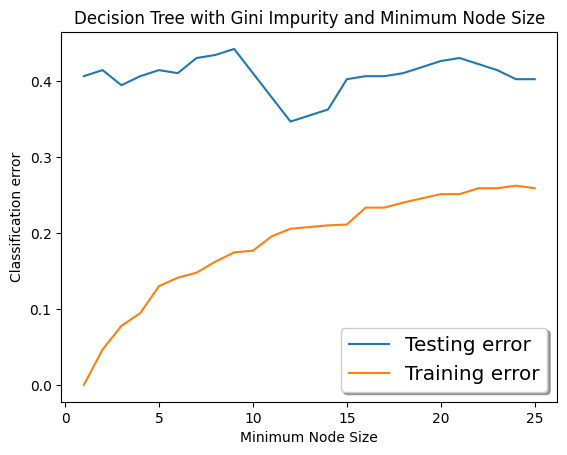
\includegraphics[width=12cm]{images/P2_A_i.png} \\
\end{solution}

\problem[6]
For either the minimal leaf node size or maximum depth parameters in the previous problem, which parameter value minimizes the test error? What effects does early stopping have on the performance of a decision tree model?
Please justify your answer based on the plot you derived.

\begin{solution}
   The minimal leaf node size parameter minimizes the test error with min_samples_leaf = 12 producing a test error of around 0.346614. The plot shows how early stopping can decrease the test error of a decision tree model significantly as it stops overfitting. We can see from the plot that if we would have allowed the 'Minimum Node Size' parameter to go all the way to 1, we would have very low training error but a large test error. Similarly, if we allow the decision tree to go to too high of a depth, we can see that the training error will go to the zero but the test error could get worse.
\end{solution}

\indent\problem[4] Choose one of the following from i or ii: \smallskip 

\noindent i. Train a random forest classifier using Gini as the impurity measure, minimal leaf node size as early stopping criterion, and 1,000 trees in the forest. Try different node sizes from 1 to 25 in increments of 1. Then, on a single plot, plot both training and test classification error versus
leaf node size.

ii. Train a random forest classifier using Gini as the impurity measure, maximal tree depth as early stopping criterion, and 1,000 trees in the forest. Try different tree depths from 2 to 20 in increments of 1. Then, on a single plot, plot both training and test classification error versus tree depth.

\begin{solution}
    \\
    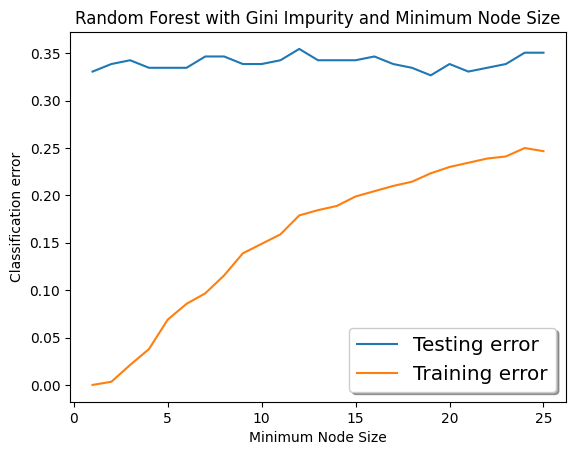
\includegraphics[width=12cm]{images/P2_C_i.png} \\
\end{solution}

\problem[6]
For either the minimal leaf node size or maximum depth parameters tested, which parameter value minimizes the random forest test error? What effects does early stopping have on the performance of a random forest model?
Please justify your answer based on the plot you derived.

\begin{solution}
    It seems that the minimal leaf node size parameter minimizes the test error with min_samples_leaf = 12 producing a test error of around 0.346614. The results of this parameter on a Random Forest are similar to that of a Decision Tree with the notable exception that the test error seems to be relatively stagnant and more consistent.
\end{solution}

\problem[4]
Do you observe any differences between the curves for the random forest and decision tree plots? If so, explain what could account for these differences.

\begin{solution}
    The Random Forest has a more consistent validation error than the Decision Tree, and this makes sense because Random Forests attempt to reduce the variance of Decision Trees by being the average of many Decision Trees. This results in a more consistent validation error and a model that is less prone to overfitting than a regular Decision Tree.
\end{solution}

\textbf{Extra Credit [7 points total] :} \problem\textbf{[5 points, Extra Credit]} Complete the other option for \textbf{Problem A }and \textbf{Problem C}.

\begin{solution}
    \\
    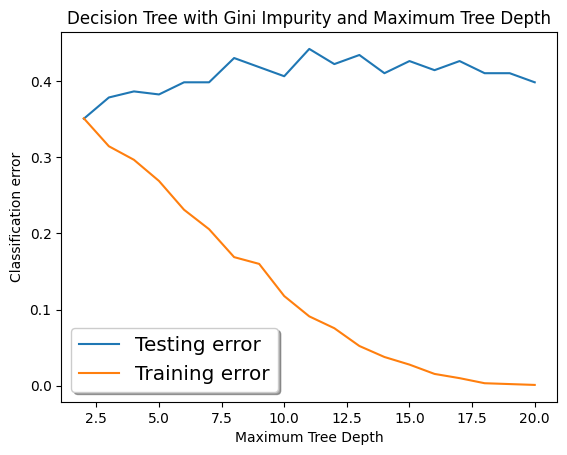
\includegraphics[width=12cm]{images/P2_A_ii.png} \\
    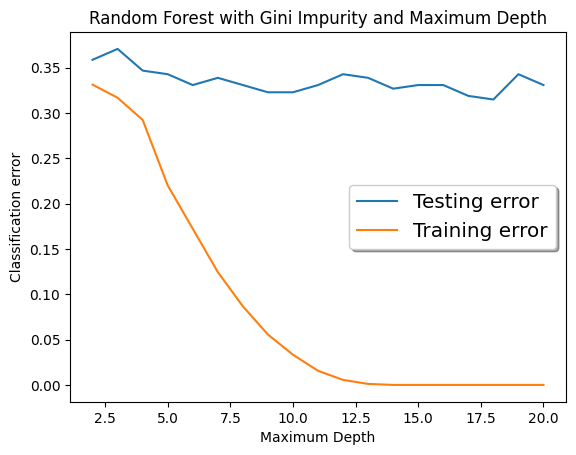
\includegraphics[width=12cm]{images/P2_C_ii.png} \\
\end{solution}

\problem\textbf{[2 points, Extra Credit] }For the stopping criterion tested in \textbf{Problem F}, which parameter value minimizes the decision tree and random forest test error respectively? 

\begin{solution}
    For the maximum depth parameter using a Decision Tree, max_depth = 2 produces a minimum test error of around 0.350598. For the maximum depth parameter using Random Forests, max_depth = 18 produces a minimum test error of around 0.314741.
\end{solution}

%%%%%%%%%%%%%%%%%%%%%%%%%%%%%%
% PROBLEM 3
%%%%%%%%%%%%%%%%%%%%%%%%%%%%%%

\newpage
\section{The AdaBoost Algorithm [40 points]}
\materials{Lecture 6}

In this problem, you will show that the choice of the $\alpha_t$ parameter in
the AdaBoost algorithm corresponds to greedily minimizing an exponential upper
bound on the loss term at each iteration.

\problem[3]
Let $h_t: \mathbb{R}^m \rightarrow \{-1,1\}$ be the weak classifier obtained at step $t$, and let $\alpha_t$ be
its weight. Recall that the final classifier is $$H(x) = \text{sign}(f(x)) = \text{sign} \left(\sum\limits_{t=1}^T \alpha_{t}h_t(x) \right).$$

Suppose $\{(x_1, y_1), ..., (x_N, y_N)\} \subset \mathbb{R}^m \times \{-1,1\}$ is our training dataset.  Show that the training set error of the final classifier can be bounded from
above if an an exponential loss function is used:

$$E = \frac{1}{N} \sum\limits_{i=1}^N \exp(-y_{i}f(x_i)) \geq \frac{1}{N} \sum\limits_{i=1}^N \mathbbm{1}(H(x_i) \neq y_i),$$

where $\mathbbm{1}$ is the indicator function.

\begin{solution}
    We will look at each element $x_i$ and show that the exponential loss is greater than the indicator loss. For each $x_i$, there are two cases: (1) the point is correctly classified $(H(x_i) = y_i)$ or (2) it is incorrectly classified $(H(x_i) \neq y_i)$. \\
    Let $I(x_i)$ = $\mathbbm{1}(H(x_i) \neq y_i)
    \text{ and let } E(x_i) = \exp(-y_{i}f(x_i))$ \\
    For the (1) case: We have that $I(x_i) = 0 \leq \exp(-y_{i}f(x_i)) = E(x_i)$ since the exponential function is always positive. \\
    For the (2) case: We have that $I(x_i) = 1$ and note that $-y_{i}f(x_i) >= 0$ since $y_{i}$ and $f(x_i)$ are of opposite signs. This implies that $E(x_i) = \exp(-y_{i}f(x_i)) \geq e^0 = 1 = I(x_i)$. \\
    In either case, we have that $E(x_i) \geq I(x_i)$ for all $x_i$, and thus we now know that the final classifier is bounded above by the exponential loss function. 
\end{solution}

\problem[3]
Find $D_{T + 1}(i)$ in terms of $Z_t$, $\alpha_t$, $x_i$, $y_i$, and the classifier $h_t$, where $T$ is the last timestep and $t \in \{1, \ldots, T\}$. Recall that $Z_t$ is the normalization factor for distribution $D_{t+1}$:
$$Z_t = \sum\limits_{i=1}^N D_t(i) \exp(-\alpha_{t}y_{i}h_{t}(x_{i})).$$

\begin{solution}
    \\
    \begin{align*}
        D_{T + 1}(i) =& \ \ \frac{D_T(i) \exp(-\alpha_{T}y_{i}h_{T}(x_{i}))}{Z_{T}} \\ 
        =& \ \ \frac{D_{T-1}(i) \exp(-\alpha_{T-1}y_{i}h_{T-1}(x_{i}))}{Z_{T-1}} \cdot \frac{\exp(-\alpha_{T}y_{i}h_{T}(x_{i}))}{Z_T} \\
        \vdots \\
        =& \ \ D_{1}(i) \cdot \frac{\exp(-\alpha_{1}y_{i}h_{1}(x_i))}{Z_1} \times \dots \times \frac{\exp(-\alpha_{T}y_{i}h_{T}(x_{i}))}{Z_T} \\
        =& \ \ D_{1}(i) \cdot \prod_{j = 1}^{T} \frac{\exp(-\alpha_{j}y_{i}h_{j}(x_i))}{Z_{j}} \\
        =& \ \ \frac{1}{N} \cdot \prod_{t = 1}^{T} \frac{\exp(-\alpha_{t}y_{i}h_{t}(x_i))}{Z_{t}}
    \end{align*} \\
    where $Z_{t} = \sum\limits_{i=1}^N D_t(i) \exp(-\alpha_{t}y_{i}h_{t}(x_{i}))$ \\
\end{solution}

\problem[2]
Show that $E = \sum_{i=1}^N  \frac{1}{N} e^{\sum_{t=1}^T -\alpha_t y_i h_t(x_i)}.$

\begin{solution}
    \begin{align*}
        E &= \frac{1}{N} \sum\limits_{i=1}^N \exp(-y_{i}f(x_i)) \\
        E &= \frac{1}{N} \sum\limits_{i=1}^N \exp(-y_{i}\cdot\sum\limits_{t=1}^T \alpha_{t}h_{t}(x_i)) \\
        E &= \sum\limits_{i=1}^N \frac{1}{N} e^{\sum\limits_{t=1}^T -\alpha_{t}y_{i}h_{t}(x_i)}
    \end{align*}
\end{solution}

\problem[5]
Show that
$$E = \prod\limits_{t=1}^T Z_t.$$

\begin{hint}
	Recall that $\sum_{i = 1}^N D_t(i) = 1$ because $D$ is a distribution.
\end{hint}

\begin{solution}
    From Problem B, we start with and simplify from:
    \begin{align*}
        D_{T+1}(i) &= \frac{1}{N} \cdot \prod_{t = 1}^{T} \frac{\exp(-\alpha_{t}y_{i}h_{t}(x_i))}{Z_{t}} \\
        &= \frac{1}{N} \cdot \frac{\exp(\sum_{t=1}^{T}-\alpha_{t}y_{i}h_{t}(x_i))}{\prod_{t = 1}^{T}Z_{t}} \\
        &= \frac{1}{N} \cdot \frac{\exp(-y_{i}f(x_i))}{\prod_{t = 1}^{T}Z_{t}} \\
        \textit{Getting the sum of all the $D_{T+1}(i)$ for all i: } \\
        1 = \sum_{i=1}^{N} D_{T+1}(i) &= \sum_{i=1}^{N} \frac{1}{N} \cdot \exp(y_{i}f(x_i)) \\
        &= \frac{1}{\prod_{t = 1}^{T}Z_{t}} \cdot E \\
        \implies E &= \prod_{t = 1}^{T}Z_{t}
    \end{align*}

\end{solution}

\problem[5]
Show that the normalizer $Z_t$ can be written as
\[Z_t = (1 - \epsilon_t) \exp(-\alpha_t) + \epsilon_{t} \exp(\alpha_t)\]
where $\epsilon_t$ is the training set error of weak classifier $h_t$ for the weighted dataset:
\[\epsilon_t = \sum\limits_{i=1}^N D_t(i)\mathbbm1(h_t(x_i) \neq y_i).\]

\begin{solution}
    \\
    From what was given: $Z_{t} = \sum_{i=1}^{N} D_{t}(i)\exp(-\alpha_{t}y_{i}h_{t}(x_i))$. We know that $y_{i}h_{t}(x_i)$ is either going to be equal to $+1$ or $-1$ Depending on whether $h_{t}(x_i) = y_{i}$ or not. So we can say:
     $$Z_{t} = \sum_{i=1 \ : \ h_{t}(x_i) = y_{i}}^{N} D_{t}(i)\exp(-\alpha_{t} \cdot 1) + \sum_{i=1 \ : \ h_{t}(x_i) \neq y{i}}^{N} D_{t}(i)\exp(-\alpha_{t} \cdot -1)$$
     For any given element $x_i$, we can know which category it should be placed into by using the classifier of the $\mathbbm1(h_t(x_i) \neq y_i)$ function. Rewritting $Z_{t}$ we get:
    \begin{align*}
        Z_{t} &= \sum_{i = 1}^{N} D_{t}(i)\exp(-\alpha_{t})\cdot\mathbbm1(h_t(x_i) = y_i) + \sum_{i = 1}^{N} D_{t}(i)\exp(\alpha_{t})\cdot\mathbbm1(h_t(x_i) \neq y_i) \\
        &= \exp(-\alpha_{t})\sum_{i = 1}^{N} D_{t}(i)\mathbbm1(h_t(x_i) = y_i) + \exp(\alpha_{t})\sum_{i = 1}^{N} D_{t}(i)\mathbbm1(h_t(x_i) \neq y_i)
    \end{align*}
    Looking at the sums of $D_{t}(i)\mathbbm1(h_t(x_i) = y_i)$ and $D_{t}(i)\mathbbm1(h_t(x_i) \neq y_i)$ we see that they are complements and we also know that $\sum_{i = 1}^{N} D_{t}(i) = 1$. So if we let $\epsilon_{t} = \sum_{i = 1}^{N} D_{t}(i)\mathbbm1(h_t(x_i) \neq y_i)$, then we know that $\sum_{i = 1}^{N} D_{t}(i)\mathbbm1(h_t(x_i) = y_i) = 1 - \epsilon_{t}$. Substituting this into the equation for $Z_{t}$, we get that: $$Z_{t} = (1 - \epsilon_{t})\exp(-\alpha_{t}) + \epsilon_{t}\exp(\alpha_{t})$$ 
\end{solution}

\problem[2]
We derived all of this because it is hard to directly minimize the training set error, but we can greedily minimize the upper bound $E$ on this error. Show that choosing $\alpha_t$
greedily to minimize $Z_t$ at each iteration leads to the choices in
AdaBoost:
$$\alpha_{t}^* = \frac{1}{2} \ln \left(\frac{1 - \epsilon_t}{\epsilon_t} \right).$$

\begin{solution}
    To greedily minimize $Z_t$, we just try to find where $\frac{\partial{Z_{t}}}{\partial{\alpha_{t}}} = 0$.
    \begin{align*}
        0 = \frac{\partial{Z_t}}{\partial{\alpha_t}} &= -(1 - \epsilon_{t})\exp(-\alpha_{t}) + \epsilon_{t}\exp(\alpha_{t}) \\
        (1 - \epsilon_{t})\cdot{e^{-\alpha_{t}}} &= \epsilon_{t}\cdot{e^{\alpha_{t}}} \\
        \frac{1-\epsilon_{t}}{e_{t}} &= e^{2\alpha_{t}} \\
        \implies \alpha_{t}^* &= \frac{1}{2}\ln(\frac{1 - \epsilon_t}{\epsilon_t})
    \end{align*}
\end{solution}

\begin{problem}[14]
    Implement the \texttt{GradientBoosting.fit()} and \texttt{AdaBoost.fit()} methods in the notebook provided for you. Some important notes and guidelines follow:
    \begin{itemize}
        \item For both methods, make sure to work with the class attributes provided to you. Namely, after \texttt{GradientBoosting.fit()} is called, \texttt{self.clfs} should be appropriately filled with the \texttt{self.n_clfs} trained weak hypotheses. Similarly, after \texttt{AdaBoost.fit()} is called, \texttt{self.clfs} and \texttt{self.coefs} should be appropriately filled with the \texttt{self.n_clfs} trained weak hypotheses and their coefficients, respectively.
        \item \texttt{AdaBoost.fit()} should additionally return an $(N, T)$ shaped numpy array \texttt{D} such that \texttt{D[:, t]} contains $D_{t+1}$ for each $t \in \{0, \ldots, \texttt{self.n_clfs}\}$.
        \item For the \texttt{AdaBoost.fit()} method, \textbf{use the 0/1 loss} instead of the exponential loss.
	\item The only Sklearn classes that you may use in implementing your boosting fit functions are the DecisionTreeRegressor and DecisionTreeClassifier, not GradientBoostingRegressor.
    \end{itemize}
\end{problem}

\begin{problem}[2]
    Describe and explain the behaviour of the loss curves for gradient boosting and for AdaBoost. You should consider two kinds of behaviours: the smoothness of the curves and the final values that the curves approach.
\end{problem}

\begin{solution}
  \\
  \url{https://colab.research.google.com/drive/1FC8WW9WLNmHabO2O83KtqNnRkLfPf6U_} \\
  Gradient Boost Loss Curve: \\
  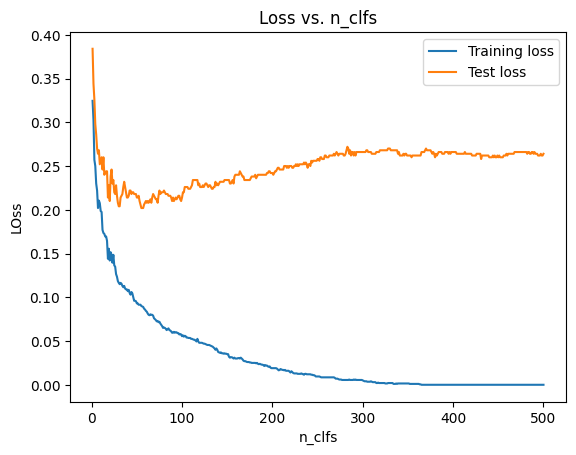
\includegraphics[width=12cm]{images/P3_H_grad_boost.png} \\
  \\ \\ \\ \\ \\ \\ \\ \\AdaBoost Loss Curve: \\
  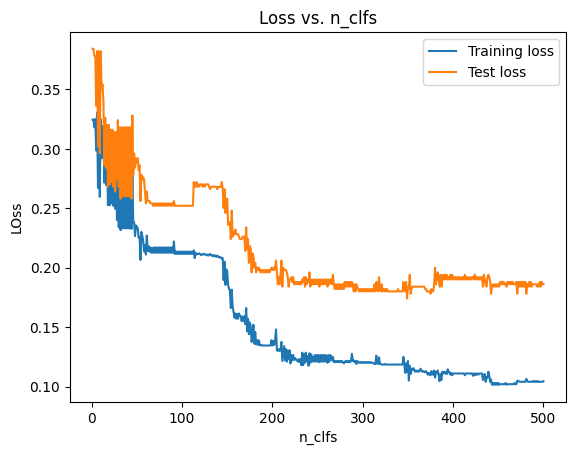
\includegraphics[width=12cm]{images/P3_H_AdaBoost.png} \\
  The Gradient Boosting Model is smoother than the AdaBoost Model and this is likely due to Gradient Boosting using Regression values and Gradient Descent which provide gradual changes in its weights. In contrast, AdaBoost predicts classification values which makes it so that its predictions are blunter and more extreme. The Gradient Boosting Model gets a lower training error ($\approx 0.00$) than the AdaBoost Model ($\approx 0.10$) but a validation error of about $36\%$ more than AdaBoost ($\approx 0.19$ for AdaBoost and $\approx 0.26$ for Gradient Boosting). This coupled with the fact that Gradient Boosting achieves its lowest validation error after only around 100 clfs implies that Gradient Boosting is a more robust algorithm than AdaBoost and was overfitting when the number of clfs increased near the end. In contrast, AdaBoost appears to have plateaued from around 200 clfs.
\end{solution}

\begin{problem}[2]
    Compare the final loss values of the two models. Which performed better on the classification dataset?
\end{problem}

\begin{solution}
    Gradient Boosting performed better on the training data set, being able to get little to no training error, however, AdaBoost performed much better than Gradient Boosting on the validation set. This is likely due to overfitting during Gradient Boosting with so many cfls. If we took the best validation error from both models though, Gradient Boosting with around 100 clfs performs about as well the final AdaBoost Model with 500 clfs.
\end{solution}

\begin{problem}[2]
    For AdaBoost, where are the dataset weights the largest, and where are they the smallest?
\end{problem}
\begin{hint}
    Watch how the dataset weights change across time in the animation.
\end{hint}
\begin{solution}
   Where AdaBoost is most jagged and has jumps, like in the beginning of training, is where the weights are largest. This makes sense because at the beginning of training, there is a lot more variance and information to learn than near the end where only minor changes to the weights are being made, seen through how there is little change in the error between adding clfs.
\end{solution}

%%%%%%%%%%%%%%%%%%%%%%%%%%%%%%
% PROBLEM 4
%%%%%%%%%%%%%%%%%%%%%%%%%%%%%%

\newpage
\section{Convex Functions [7 points, EC 3 Points]}

\emph{This problem further develops the ideas of convex functions, and provides intuition for why convex optimization is so important for
 Machine Learning.}

Given a convex set $\mathcal{X}$, a function $f:\mathcal{X}\to\mathbb{R}$ is \textbf{convex} if for all $\textbf{x},\textbf{y}\in \mathcal{X}$ and all $t\in[0,1]$ :
\[f(t\textbf{x} + (1-t)\textbf{y}) \leq tf(\textbf{x}) + (1-t)f(\textbf{y})\]

\begin{problem}[3]
Let $\mathcal{X}$ be a convex set. If $f$ is a convex function, show that any local minimum of $f$ in $\mathcal{X}$ is also a global minimum.
\end{problem}

\begin{solution}
    Let $\hat{x}$ be a local minimum in $\mathcal{X}$ and let $x' \neq \hat{x}$ be the global minimum of $\mathcal{X}$. The line between the two points is in $\mathcal{X}$ by definition and can be denoted by: $x(t) = t\hat{x} + (1 - t)x'$. Because $f$ is a convex function on $\mathcal{X}$, we know that $$ f(x(t)) \leq tf(\hat{x}) + (1 - t)f(x') < f(\hat{x}) $$ since $ 0 \leq t < 1$ and $f(x') < f(\hat{x})$. Now, note that if we let $\lim_{t \to 0} x(t)$, we get that points near $\hat{x}$ are less than $\hat{x}$, which is a contradiction since $\hat{x}$ is a local minimum. Therefore, we know that there cannot exist an $x' \neq \hat{x}$ which is a global minimum, and it must be the case that $x' = \hat{x}$ is the global minimum on $\mathcal{X}$.
\end{solution}

\begin{problem}[4]
\emph{Using part A}, explain why convex loss functions are desirable when training learning models.
\end{problem}

\begin{solution}
    Convex loss functions are desirable for training learning models because a learning model usually is trained to minimize its loss locally without knowing whether it is going toward a global or local minimum. However, if we know that any minimum we find will be the global minimmum, then we do not have to worry about getting stuck in a pit and can know that the solution that we are approximating is the best solution.
\end{solution}
\problem\textbf{[3 points, Extra Credit] }
The Kullback-Leibler (KL) divergence is a measure of statistical distance between two probability distributions $(p, q)$, also called the relative entropy. KL divergence can be used to generate optimal parameters for visualization models (which we will also see in set 4).
\[\mathrm{KL}[P\|Q] = \sum_{x\in\mathcal{X}} p(x) \cdot \log \frac{p(x)}{q(x)}\]
Show that the KL divergence is a convex loss function. \\

\begin{hint}
    Use the log sum inequality
\end{hint}

\begin{solution}
   
\end{solution}
\end{document}